\documentclass{beamer}
\usepackage{../tut-slides}
\usepackage{../mathoperatorsAuD}

\usepackage{lmodern}
\usepackage{amsmath,amssymb}
\usepackage{stmaryrd}
\usepackage{enumerate}
%\usepackage[inline]{enumitem} 		%customize label
%\newcommand{\labelitemi}{\raisebox{1pt}{\scalebox{.9}{$\blacktriangleright$}}}
%\newcommand{\labelitemii}{$\vartriangleright$}
%\newcommand{\labelitemiii}{--}
\setbeamertemplate{itemize item}{\raisebox{1pt}{\scalebox{.9}{$\blacktriangleright$}}}
\setbeamertemplate{itemize subitem}{$\vartriangleright$}

\usepackage{booktabs}
\usepackage{tabularx}
\usepackage{tabu}
\newcommand*\head{\rowfont{\bfseries}}
\newcommand*{\tw}{\rowfont{\ttfamily}}
\renewcommand{\tabularxcolumn}[1]{>{\hspace{0pt}}m{#1}}
\usepackage{multirow}

\usepackage{cancel}

\usepackage{empheq}
\newcommand*\widefbox[1]{\fbox{\hspace{2em} #1 \hspace{2em}}}

\usepackage{tcolorbox}
\newtcolorbox{mymathbox}[1][]{colback=white, sharp corners, #1}

\usepackage{xcolor}
\usepackage{listings}
\newcommand*{\ttfamilywithbold}{\fontfamily{lmtt}\selectfont}
\lstset{numbers=left, 
	numberstyle=\tiny, 
	breaklines=true,
	backgroundcolor=\color{cdgray!10},
	numbersep=5pt,
	language=C,
	tabsize=2,
	basicstyle=\ttfamilywithbold,
	showstringspaces=false} 
\lstdefinestyle{example}{
	basicstyle=\footnotesize\ttfamilywithbold,   
	breakatwhitespace=false,         % sets if automatic breaks should only happen at whitespace
	breaklines=true,                 % sets automatic line breaking
	commentstyle=\itshape,    	     % comment style
	escapeinside={\%*}{*)},          % if you want to add LaTeX within your code
	extendedchars=true,              % lets you use non-ASCII characters; for 8-bits encodings only, does not work with UTF-8
	backgroundcolor=\color{cdgray!10},
	keywordstyle=\bfseries,       % keyword style
	morekeywords={}, 
	language=C,                 % the language of the code
	numbers=none,                    % where to put the line-numbers; possible: (none, left, right)
	numbersep=5pt,                   % how far the line-numbers are from the code
	numberstyle=\tiny\color{cdgray!50}, % the style that is used for the line-numbers
	rulecolor=\color{cddarkblue}, 
	tabsize=2,	                   % sets default tabsize to 2 spaces
}

\DeclareMathOperator{\ack}{\mathbf{ack}}
\usepackage{MnSymbol}

\newcommand{\col}[1]{\textcolor{cdpurple}{#1}}
\newcolumntype{R}[1]{>{\centering\arraybackslash}p{#1}}

\usepackage{csquotes}

%%%% EBNF-Terme %%%%
\usepackage{../syntaxdiagrammEBNF}

\begin{document}	
	\title{Algorithmen und Datenstrukturen}
	\subtitle{Übung 5: Funktionen \& Pulsierender Speicher}
	\author{Eric Kunze}
	\email{eric.kunze@tu-dresden.de}
	\city{TU Dresden}
%	\institute{Lehrstuhl für Grundlagen der Programmierung}
	\titlegraphic{
\includegraphics[width=2cm]{../TUD-white.pdf}}
	\date{\today}

	\maketitle


%%%%%%%%%%%%%%%%%%%%%%%%%%%%%%%%%%%%%%%%%%%%%%%%%%%%%%%%%%%%%%%%%%%%%%%%%%%%%

%%%%%%%%%%%%%%%%%%%%%%%%%%%%%%%%%%%%%%%%%%%%%%%%%%%%%%%%%%%%%%%%%%%%%%%%%%%%%%%%%%%

\begin{frame} \frametitle{Pulsierender Speicher}
	\small
	\textbf{Gültigkeitsbereiche von Objekten}:
	\begin{itemize}
		\item Eine Funktion ist ab ihrer Deklaration bis zum Programmende sichtbar. Vorwärtsdeklarationen beachten!
		\item  Ihre formalen Parameter jedoch nur innerhalb der Funktionsdefinition!
		\item Gibt es gleichlautende formale Parameter in verschiedenen Funktionen, müssen diese in der Tabelle natürlich unterschieden werden (z.B. durch \enquote{x in f}).
		\item Vorsicht bei Namenskonflikten: lokale Variablen überschreiben die Sichtbarkeit globaler Variablen.
	\end{itemize}
\end{frame}

\begin{frame} \frametitle{Pulsierender Speicher}
	\small
	\textbf{Speicherprotokoll}:
	\begin{itemize}
		\item Für jeden Funktionsaufruf werden erst die Parameter, dann die lokalen Variablen in Reihenfolge ihres Auftretens in der Umgebung notiert. Globale Variablen stehen ganz vorn.
		\item Variablennamen werden nur notiert, wenn die Variablen sichtbar sind. Globale Variablennamen werden immer notiert.
		\item Der Wert von nicht sichtbaren Variablen muss nur notiert werden wenn er sich ändert.
		\item Uninitialisierte Variablen werden mit Inhalt \enquote{?} notiert.
	\end{itemize}
\end{frame}

\begin{frame} \frametitle{Aufgabe 3}
	\centering
	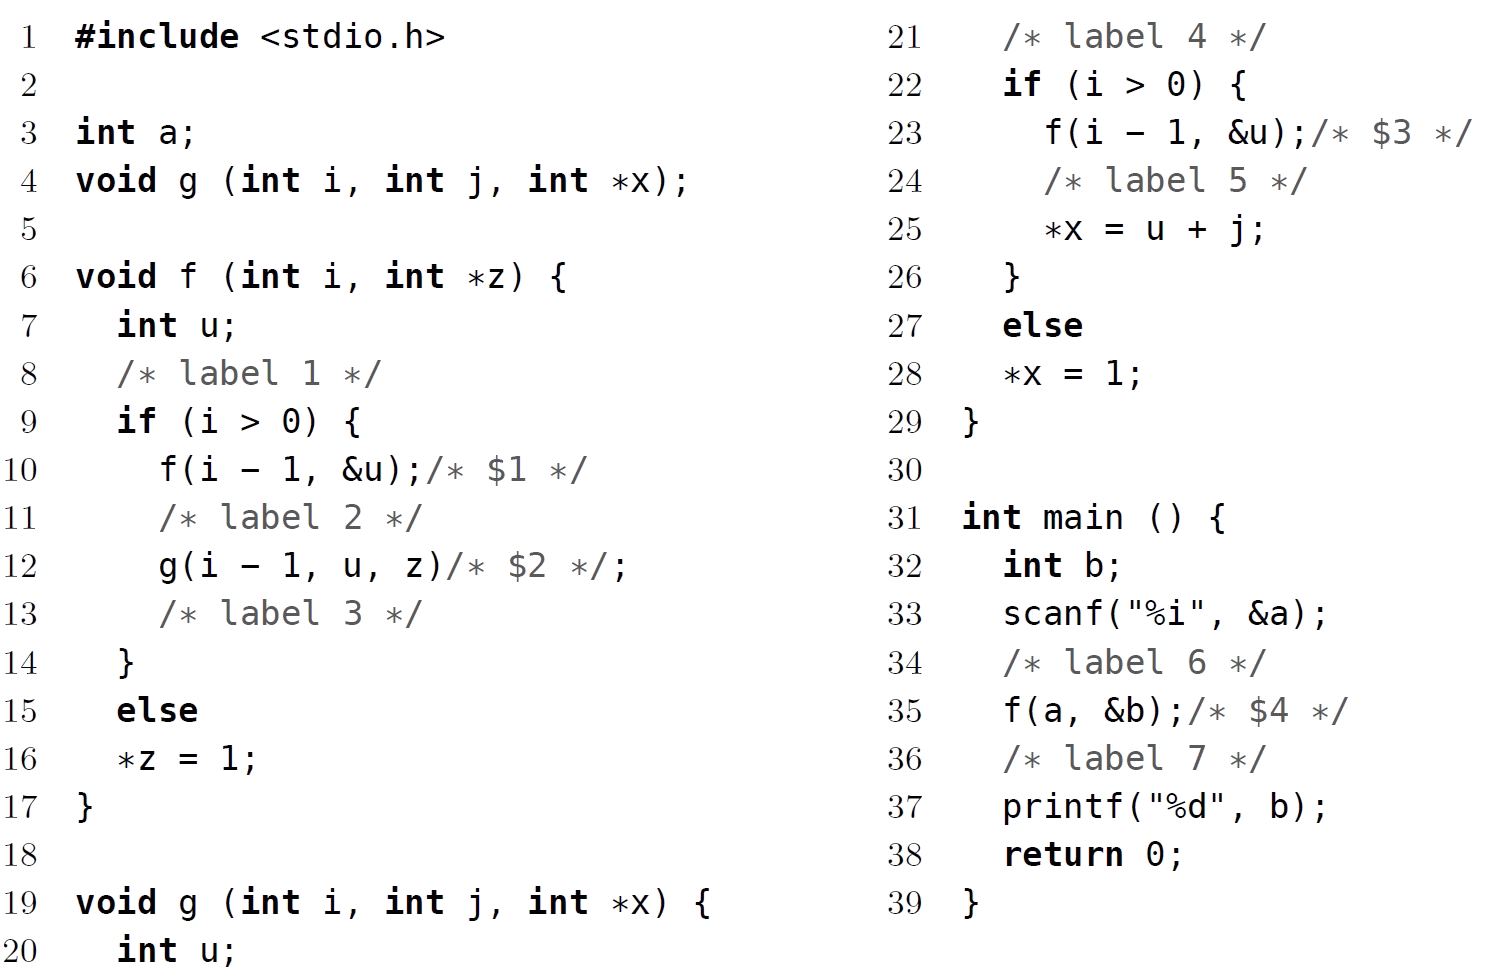
\includegraphics[width=\textwidth]{./tut05_aufgabe3.png}
\end{frame}

\begin{frame} \frametitle{Aufgabe 3 --- Teil (a)}
	\textbf{Gültigkeitsbereiche}

	\centering
	\begin{tabular}{|l|c|}
		\hline
		Objektname & Gültigkeitsbereich \\ \hline \hline
		\texttt{a} & 2 -- 14 und 25 -- 33 \\ \hline
		\texttt{g} & 4 -- 33 \\ \hline
		\texttt{a, b} in \texttt{g} & 15 -- 24 \\ \hline
		\texttt{i} in \texttt{g} & 16 -- 24 \\ \hline
		\texttt{f} & 6 -- 33 \\ \hline
		\texttt{i,j} in \texttt{f} & 6 -- 13 \\ \hline
		\texttt{main} & 26 -- 33 \\ \hline
		\texttt{x} in \texttt{main} & 27 -- 33 \\ \hline
	\end{tabular}
\end{frame}


\begin{frame} \frametitle{Aufgabe 3 --- Teil (b)}
	\centering
	\scalebox{0.6}{
	\def\arraystretch{0.9}
	\begin{tabular}{|p{2.5cm}|p{2cm}||R{0.5cm}||R{0.5cm}|R{0.5cm}|R{0.5cm}|R{0.5cm}|R{0.5cm}|R{0.5cm}|R{0.5cm}|R{0.5cm}|R{0.5cm}|R{0.5cm}|R{0.5cm}|}
		\hline
		Label & RM & 1 & 2 & 3 & 4 & 5 & 6 & 7 & 8 & 9 & 10 & 11 & 12 \\ 
		\hline \hline
		 &       &  &  &   &   &   &   &   &   &   &   &   & \\ 
	           &         &  &  &   &   &   &   &   &   &   &   &   & \\ \hline
		 &       &   &   &  &  & &   &   &   &   &   &   & \\ 
		       &         &   &   &  &  &  &   &   &   &   &   &   & \\ \hline
		 &     &  &   &   &   &   &  &  &   &   &   &   & \\ 
		       &         &  &   &   &   &   &  & &   &   &   &   & \\ \hline
		 &      &  &   &   &   &   &  &  &   &   &   &   & \\ 
			   &         &  &   &   &   &   &  & &   &   &   &   & \\ \hline
		 &        &   &   &  &  &  &   &   &   &   &   &   & \\ 
			   &         &   &  &  &  &  &   &   &   &   &   &   & \\ \hline
		 &      &  &   &   &   &   &  &  &   &   &   &   & \\ 
		       &         &  &   &   &   &   &  &  &   &   &   &   & \\ \hline
		 &    &  &   &   &   &   &   &   &  &  &   &   & \\ 
			   &         & &   &   &   & &   &   &  &  &   &   & \\ \hline
		 &  &  &   &   &   &   &   &   &   &   &  &  & \\ 
			   &         & &   &   &   &  &   &   &   &   &  &  & \\ \hline
		 &  &  &   &   &   &   &   &   &   &   &  &  & \\ 
			   &         &  &   &   &   &   &   &   &   &   &  &  & \\ \hline
		 &   &  &   &   &   &   &   &   &  &  &   &   & \\ 
		       &         &  &   &   &   &   &   &   &  &  &   &   & \\ \hline
		 &     &  &   &   &   &   &  &  &   &   &   &   & \\ 
		       &         &  &   &   &   &   &  &  &   &   &   &   & \\ \hline
		 &        &   &   &  &  &  &   &   &   &   &   &   & \\ 
			   &         &   &  &  &  &  &   &   &   &   &   &   & \\ \hline
		 &       &  &  &   &   &   &   &   &   &   &   &   & \\ 
			   &         &  &  &   &   &   &   &   &   &   &   &   & \\ \hline
	\end{tabular}}
\end{frame}

\begin{frame} \frametitle{Aufgabe 3 --- Teil (b)}
	\centering
	\scalebox{0.6}{
		\def\arraystretch{0.9}
		\begin{tabular}{|p{1cm}|r||R{0.5cm}||R{0.5cm}|R{0.5cm}|R{0.5cm}|R{0.5cm}|R{0.5cm}|R{0.5cm}|R{0.5cm}|R{0.5cm}|R{0.5cm}|R{0.5cm}|R{0.5cm}|}
			\hline
			Label & RM & 1 & 2 & 3 & 4 & 5 & 6 & 7 & 8 & 9 & 10 & 11 & 12 \\ 
			\hline \hline
			label5 & --      & a & x &   &   &   &   &   &   &   &   &   & \\ 
			&         & 7 & 0 &   &   &   &   &   &   &   &   &   & \\ \hline
			label3 & 3       &   &   & a & b & i &   &   &   &   &   &   & \\ 
			&         &   &   & 7 & 2 & 2 &   &   &   &   &   &   & \\ \hline
			label1 & 2:3     & a &   &   &   &   & i & j &   &   &   &   & \\ 
			&         & 7 &   &   &   &   & 5 & 7 &   &   &   &   & \\ \hline
			label2 & 2:3     & a &   &   &   &   & i & j &   &   &   &   & \\ 
			&         & 7 &   &   &   &   & 5 & 7 &   &   &   &   & \\ \hline
			label4 & 3       &   &   & a & b & i &   &   &   &   &   &   & \\ 
			&         &   & 1 & 3 & 2 & 2 &   &   &   &   &   &   & \\ \hline
			label1 & 2:3     & a &   &   &   &   & i & j &   &   &   &   & \\ 
			&         & 7 &   &   &   &   & 5 & 3 &   &   &   &   & \\ \hline
			label1 & 1:2:3   & a &   &   &   &   &   &   & i & j &   &   & \\ 
			&         & 7 &   &   &   & 3 &   &   & 5 & 3 &   &   & \\ \hline
			label1 & 1:1:2:3 & a &   &   &   &   &   &   &   &   & i & j & \\ 
			&         & 7 &   &   &   & 4 &   &   &   &   & 5 & 3 & \\ \hline
			label2 & 1:1:2:3 & a &   &   &   &   &   &   &   &   & i & j & \\ 
			&         & 7 &   &   &   &   &   &   &   &   & 5 & 3 & \\ \hline
			label2 & 1:2:3   & a &   &   &   &   &   &   & i & j &   &   & \\ 
			&         & 7 &   &   &   &   &   &   & 5 & 3 &   &   & \\ \hline
			label2 & 2:3     & a &   &   &   &   & i & j &   &   &   &   & \\ 
			&         & 7 &   &   &   &   & 5 & 3 &   &   &   &   & \\ \hline
			label4 & 3       &   &   & a & b & i &   &   &   &   &   &   & \\ 
			&         &   & 2 & 1 & 2 & 4 &   &   &   &   &   &   & \\ \hline
			label6 & --      & a & x &   &   &   &   &   &   &   &   &   & \\ 
			&         & 7 & 2 &   &   &   &   &   &   &   &   &   & \\ \hline
	\end{tabular}}
\end{frame}




%%%%%%%%%%%%%%%%%%%%%%%%%%%%%%%%%%%%%%%%%%%%%%%%%%%%%%%%%%%%%%%%%%%%%%%%%%%%%%%%%%%

\end{document}